\documentclass[tikz, border=1cm, convert={density=300,outext=.png}]{standalone}
\usetikzlibrary{backgrounds}

\begin{document}

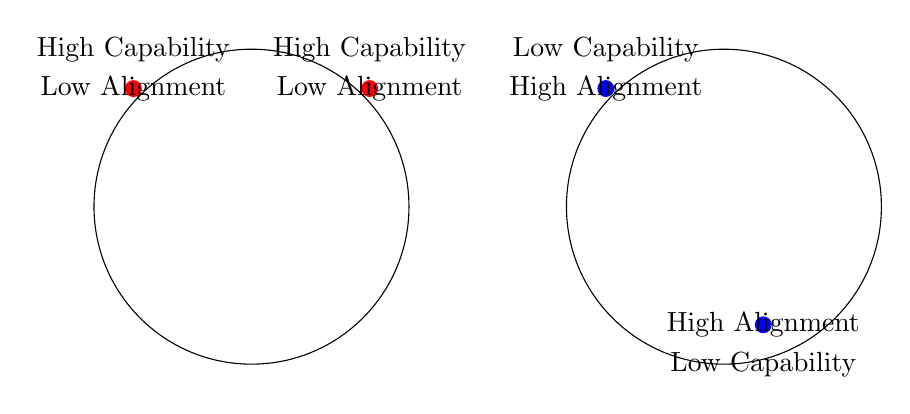
\begin{tikzpicture}

    % draw circles
    \draw[black, fill=white] (0,0) circle (2cm);
    \draw[black, fill=white] (6,0) circle (2cm);
    
    % draw points
    \draw[red, fill=red] (-1.5,1.5) circle (0.1cm);
    \draw[red, fill=red] (1.5,1.5) circle (0.1cm);
    \draw[blue, fill=blue] (4.5,1.5) circle (0.1cm);
    \draw[blue, fill=blue] (6.5,-1.5) circle (0.1cm);
    
    % add labels
    \node at (-1.5,2) {High Capability};
    \node at (-1.5,1.5) {Low Alignment};
    \node at (1.5,2) {High Capability};
    \node at (1.5,1.5) {Low Alignment};
    \node at (4.5,2) {Low Capability};
    \node at (4.5,1.5) {High Alignment};
    \node at (6.5,-2) {Low Capability};
    \node at (6.5,-1.5) {High Alignment};
    
\end{tikzpicture}

\end{document}
